\chapter{Methods and Approach}
    \label{approach}

I evaluate the Uncertainty-Aware Deep Q-Network (UA-DQN) algorithm empirically for the task of building energy control.
The experiment is realized using CityLearn to construct the reinforcement learning environment, using data from the 2022 CityLearn challenge.
As a baseline, I establish a rule-based policy based on patterns in the data.
Finally, I compare UA-DQN against the baseline and two versions of the DQN algorithm that differ in their action selection.


\section{Environment}
The Reinforcement Learning environment used by the experiments in this thesis is based on the 2022 CityLearn Challenge\footnote{\url{https://www.aicrowd.com/challenges/neurips-2022-citylearn-challenge}}.
The environment provides a simulation of building energy systems, along with hourly data on electricity price, usage, solar production and weather data.
The task is to control the storage and release of electricity in an electrical battery, with the objective of jointly reducing total per-building cost and carbon emissions.
In contrast to the complete challenge setup, the experiments described in this thesis only use one building.

The simulation framework used by both the challenge and this thesis is CityLearn as proposed by \citep{vazquez-canteli2019CityLearnV1OpenAI}.

\subsection{Data}
The Dataset provided for the 2022 CityLearn challenge setup contains a year of hourly observations of a number of variables that describe the energy system of a building.
At it's core, it supplies real-world per-building measurements of electricity use and photovoltaic solar power generation from five model buildings set up by the Electric Power Research Institute (EPRI) in Fontana, California as part of the research described in \cite{narayanamurthy2016GridIntegrationZero}.
Building data is coupled with weather observations (Outdoor Temperature, Relative Humidity, Diffuse and Direct Solar Radiation).
Weather forecasts are also provided, which are generated by shifting ground truth observations by an offset of 6, 12 and 24 hours.
The data also contains carbon intensity and price of electricity provided by the grid.
Time variables included are hour of the day, day of the week and month.
The source for the non-building data is unfortunately not given by the challenge organizers.

A sample day of building and price data is shown in figure \ref{fig:data}.
In building 1, daily solar production exceeds building electricity consumption on 72/365 days.

\begin{figure}
    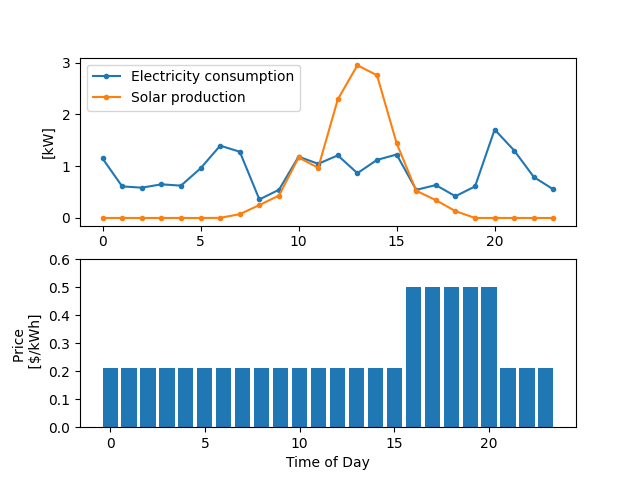
\includegraphics[width=\figurewidth]{figures/data.png}
    \caption{A sample day of electricity production, consumption and price for one building.}
    \label{fig:data}
\end{figure}

\subsection{Environment Details}
\subsubsection{Observation Space}
For this research, I make available a subset of the provided dimensions, given in table \ref{tab:observations}. Observations are dynamically normalized to zero mean and unit variance.

\begin{table}[h]
    \caption{The observed variables available in the experiments. Observations are dynamically normalized to the same scale.} \label{tab:observations}
    \centering
    \begin{tabular}{l|c}
        Variable & Unit \\ \hline
        Hour & 1-hot encoding 0-24 \\
        Direct Solar Irradiance (predicted 6h) & $W/m^2$ \\
        Carbon Intensity & $kg/kWh$ \\
        Building Electric Load & $kW$\\
        Building Solar Generation & $kW$\\
        Building Battery State of Charge & $kWh$\\
    \end{tabular}
\end{table}

\subsubsection{Action Space}
The action space provided by CityLearn is the continuous real interval $[-1,1]$, where negative actions are an attempt to discharge, and positive actions are an attempt to charge the battery.
The action is scaled in units of the battery's capacity, so -1 means an attempt to discharge the whole battery.

The actual resulting charging and discharging speeds are limited by CityLearn's energy model and depend on the battery's state of charge.

The studied Reinforcement Learning algorithms require a discrete action space.
I discretize the action space into a number of discrete actions. The number of discrete actions is determined with the experiment described in section \ref{sec:discretization}.

\subsubsection{Reward Function}
The reward function is designed to match the initial challenge objective as closely as possible.
The per-building reward at time step $t$ is given by
$$r_t = - \left(\frac{\text{cost}_t}{\text{cost}_\text{no battery total}}
    + \frac{\text{carbon emissions}_t}{\text{carbon emissions}_\text{no battery total}}\right) \cdot 8760,$$
where $()\text{cost}_\text{no battery total})$ and $(\text{carbon emissions}_\text{no battery total})$ are the total dollar cost and carbon emissions observed over one year in a control situation where the battery is never used.
The reward is always negative.

\subsection{Implementation Details}
During the 2022 CityLearn Challenge, I contributed work to the CityLearn framework.
I found and proposed a fix for an implementation error that meant that the environment would recompute the entire episode history at every time step $t$.
My fix\footnote{\url{https://github.com/intelligent-environments-lab/CityLearn/pull/23}} instead reuses the result of the preceding time step $t-1$, which changes the per-step complexity from $O(t^2)$ to $O(1)$, roughly leading to a 100x-speedup over the course of an episode.
I also contributed to finding a bug\footnote{\url{https://github.com/intelligent-environments-lab/CityLearn/issues/37}} in the battery model.
These efforts were rewarded with the Community Contribution Prize.

The software environment for all experiments uses Python 3.10.9, PyTorch 1.13.0, OpenAI gym 0.24.1, and CityLearn 1.3.6.

The hardware used was a 2020 MacBook Air M1 for the discretization pre-experiment. Tuning and subsequent evaluation runs were scheduled on a Slurm cluster, using CUDA on a single Nvidia GTX 2080 GPU per run. The Slurm job scheduling file is included in the attached code repository.


\section{Algorithm}
\subsection{Uncertainty-Aware Deep Q-Network} % the new method I want to evaluate.
In RL, it is important to distinguish between epistemic uncertainty, which is caused by limited data, and aleatoric uncertainty, which is caused by stochasticity in the environment \citep{hullermeier2021AleatoricEpistemicUncertainty}.
Efficient exploration aims to reduce epistemic uncertainty for promising actions, but can't reduce aleatoric uncertainty.
\cite{nikolov2022InformationDirectedExplorationDeep} propose to estimate aleatoric uncertainty using the variance of the estimated reward distribution.
However, \cite{chua2018DeepReinforcementLearning} highlight that this approach fails for novel, out-of-distribution data, when epistemic uncertainty is high.

The UA-DQN algorithm proposed by \cite{clements2020EstimatingRiskUncertainty} learns a distribution of expected rewards, and simultaneously provides estimates for epistemic and aleatoric uncertainties.
These uncertainties are used to adjust the expected value and variance for each action, before using Thompson sampling to select an action.
This leads to an algorithm that can efficiently explore.
Depending on its hyperparameters, the algorithm can be more or less risk-averse.

Efficient exploration and risk-aware strategies are most important when the costs and risks associated with an environment interaction are high, as they are in a real-world energy setting.
Therefore, I test the performance of the UA-DQN algorithm on the battery control environment, replicating the experiments described in \cite{clements2020EstimatingRiskUncertainty}.

\subsection{DQN}
In order to study the benefit of an explicit uncertainty treatment, I evaluate the performance of two variants of the standard DQN algorithm.
Like in \cite{clements2020EstimatingRiskUncertainty}, one DQN variant acts according to an $\epsilon$-greedy policy, which linearly decays $\epsilon$ from 1.0 to 0.02 in the first 1000 steps.
The second variant, referred to throughout the thesis as "DQN-Softmax" uses Boltzmann sampling on the estimated Q-values.

\subsection{Implementation Details}
The implementation for all three Reinforcement Learning agents is based on the implementation provided with \cite{clements2020EstimatingRiskUncertainty} with minimal changes.
All neural networks have two hidden layers with 128 neurons each and ReLU activation functions.
They are randomly initialized with an orthogonal matrix as described by \cite{saxe2014ExactSolutionsNonlinear}, with a weight scale factor of $\sqrt{2}$.

All algorithms use the Adam optimizer, with tuned $\epsilon$ and learning rate parameters.
All algorithms use experience replay and a periodically updated target Q-network.

UA-DQN is set to be risk-neutral, with the aleatoric factor fixed to 0 and the epistemic factor fixed to 1.
Loss functions are Mean Squared Error for DQN, and Quantile Huber Loss for UA-DQN.

\subsection{Baseline Rule-Based-Controller}
In order to be able to evaluate the performance of the Reinforcement Learning agent, I establish a rule-based controller as baseline.
Using insights gained from exploratory data analysis, I construct a simple control policy with the goal of minimizing dollar cost.

The basis of the policy is that prices vary predictably.
Throughout every day, electricity price is at one of two levels.
From 16:00 to 20:00, it is substantially higher than during the rest of the day.
In parts of the year, the price level also varies between different days of the week, but the daily pattern still applies.
Since battery energy losses are very low, it is therefore worth it to buy and store electricity while it's cheap, and avoid having to buy expensive electricity in the afternoon.

In addition to the electrical grid, the agent also has access to a free, but less predictable source of electricity: solar power.
The environment does not allow the agent to sell electricity for a profit.
This means any produced solar electricity should either be directly used or stored, since any excess is simply discarded.
Directly using solar electricity is more efficient than storing and releasing it at a later time.
Putting these basic ideas together, I arrive at a policy that first uses available solar electricity to meet demand.
It aims to always store excess solar electricity, and additionally buys just enough cheap electricity in order to fill up the battery for the more expensive afternoon.

Because the policy has to make a decision based on the past hour's solar production and electricity consumption, it simply assumes there's no change and tries to store the amount of excess electricity observed before.

This strategy leaves open one question:
When exactly should the battery be charged with electricity from the grid?
If it is filled too early, the agent is not able to store excess solar electricity generated during the day.
Therefore, the battery is charged as late as possible.
However, if battery charging starts too late, there is not enough time left to fully charge the battery. 
Lastly, if the battery has remaining charge after the period of high prices, the leftover charge is used as needed, ensuring the battery is free in the morning to store any excess solar power.
The final policy is described in algorithm \ref{alg:rbc}.

\begin{algorithm}[h]
    \begin{algorithmic}
        \State $a \gets (\text{solar} - \text{load})/6.4$ \Comment{Difference scaled to units of battery capacity}
        \If{$11 \leq \text{hour} \leq 15$}
            \State $a \gets \max(0.24, a)$ \Comment{Slowly charge battery}
        \EndIf
        \Ensure $-1 \leq a \leq +1$ \\
        \Return $a$
    \end{algorithmic}
    \caption{The Rule-Based Controller's Policy}
    \label{alg:rbc}
\end{algorithm}

This hand-engineered policy is not perfectly optimized.
There are certain insights it does not make use of.
It does not directly minimize carbon emissions, though the overall reduced demand for grid electricity leads to a reduction in emissions.
The policy also does not incorporate the change in price between weekdays.
There are some days on which there is so little excess demand during the day that it would not be worth charging the battery.
Finally, the policy does not make use of weather forecasts, which predict solar electricity production.

Overall, the policy is a useful benchmark of expert human performance.

\section{Experiment} % How I plan to evaluate it

\subsection{Discretization} \label{sec:discretization}
UA-DQN and DQN require a discrete action space.
In CityLearn, the action is a continuous number between -1 (releasing energy) and +1(storing energy).
Therefore, I subdivide the continuous action space into multiple discrete actions.
The goal of this pre-experiment is to determine a suitable resolution of subdivision of the continuous action space.
A larger discrete action space means the algorithm learns slower, but a smaller discrete action space means the algorithm can't act as precisely, capping the possible performance.
The goal therefore is to find the smallest number of subdivisions that does not produce a significant drop in performance.

In order to measure the importance of different subdivisions, I run the baseline rule-based policy on versions of the environment with differently discretized action spaces.
The environment uses the entire 2022 CityLearn challenge public dataset of 5 buildings and one year.

I measure the performance as calculated by CityLearn, both cost and carbon metrics.
The performance on the discretized action spaces is compared with the policy's performance on the continuous action space.

\subsection{Hyperparameter Tuning}
All tested Deep Reinforcement Learning agents and the optimizer, Adam, expose hyperparameters that need to be tuned for optimal performance.
Adam's tuned hyperparameters are the learning rate and the parameter $\epsilon$.
I also tuned the batch size and the update frequency of the target networks.
All other hyperparameters I set to default values as noted in table \ref{tab:tuning}.

\begin{table}
    \centering
    \caption{Hyperparameters, their tuning ranges or non-tuned values.}
    \label{tab:tuning}
    \begin{tabular}{l|c}
        Hyperparameter & Tuning Range / Value \\ \hline
        Learning Rate  & $(0.1, 0.07, 0.03, 0.01, 0.007,\dots, 0.00001)$\\
        Batch Size     & $(1,2,4,8,\dots ,256)$                             \\
        Adam's $\epsilon$ & $(1\times 10^{-1}, 1\times 10^{-2}, \dots, 1\times 10^{-9})$ \\
        \makecell[l]{Target Network \\ Update Frequency} & $(4, 8, 16, 32)$ \\ \hline
        Replay Buffer Size & 10,000 \\
        Discount Rate $\gamma$ & 0.99 \\
        Initialization Weight scale & $\sqrt{2}$ \\
        $\epsilon$-greedy DQN: $\epsilon$ & Decay from 1 to 0.02 over 1,000 steps \\
        UA-DQN: Quantile Huber Loss $\kappa$ & 10 \\
        UA-DQN: aleatoric factor & 0 \\
        UA-DQN: epistemic factor & 1 \\
    \end{tabular}
\end{table}

The process of tuning was to randomly sample 200 combinations of hyperparameters from the sets given in table \ref{tab:tuning} for each DQN variant, and 100 for UA-DQN.
The DQN variants ran for 100 episodes, UA-DQN ran for 50 episodes.
All runs used the same random seed.
Data used for this experiment was the whole year of building 1.

The performance measure for this experiment was the collected total reward in the last episode.
For each algorithm, I select the single best performing combination of hyperparameters from the tuning runs for further study.

\subsection{Comparison of Tuned Algorithms}
Following the analysis of \cite{clements2020EstimatingRiskUncertainty}, I measure the fraction of non-greedy actions for each algorithm during a training run of 50 episodes.
A non-greedy action is an action that does not correspond to the algorithm's highest expectation for expected total reward. Instead, it was taken in order to explore the environment rather than exploit current knowledge.
This illustrates the difference in how the algorithms balance exploitation and exploration as they learn.

Finally, I repeat the previous experiment with 10 different random seeds in order to be able to measure the repeatability and resource demands of each algorithm.
I evaluate each algorithm by its mean performance compared to the baseline and by its variance in final performance.
In order to evaluate the difference in resource use between the algorithms, I also measure the average wall clock time taken per training episode.